% !TEX root = ../main.tex

% 实验记录	
\begin{table}
	\renewcommand\arraystretch{1.7}
	\centering
	\begin{tabularx}{\textwidth}{|X|X|X|X|}
		\hline
		Major： & Physics & Grade： & 2022 \\
		\hline
		Name： & 杨舒云 & Student number： & 22344020 \\
		\hline
		Room temperature： & 26\degree C & Experimental location： & A101 \\
		\hline
		Student Signature：& \textbf{In Attachment} & Score： &\\
		\hline
		Experiment time：& 2024/10/25 & Teacher's Signature：&\\
		\hline
	\end{tabularx}
\end{table}
\section{APL1-1-A 电阻热噪声及玻尔兹曼常量测量 \\ Experimental Record}


%---------------------------------------------------------------------
% 实验过程记录
\subsection{Content, Procedures \& Results}

% 操作步骤
\subsubsection{Operations}
\begin{enumerate}
	\item 实验前的梳理与排查。
	
	\item 按讲义回顾并完成“实验1.6 滤波器带宽对输出信号响应的影响”。
	
	此处补上上次本应完成的实验1.6及其结果，后面就不再对此做讨论了。
	
	\begin{figure}[htbp]
		\centering
		\subfloat[100$\mu$s 6dB/oct]{\label{100us 6dB/oct}
			
\includegraphics[width=0.32\linewidth]{100us 6.jpg}}
		\quad
		\subfloat[100$\mu$s 12dB/oct]{\label{100us 12dB/oct}
			
\includegraphics[width=0.32\linewidth]{100us 12.jpg}}
		\quad
		\subfloat[100$\mu$s 18dB/oct]{\label{100us 18dB/oct}
			
\includegraphics[width=0.32\linewidth]{100us 18.jpg}}
		\quad
		\subfloat[100$\mu$s 24dB/oct]{\label{100us 24dB/oct2}
			
\includegraphics[width=0.32\linewidth]{100us 24.jpg}}
		\quad
		\caption{时间常数为 100$\mu$s 不变，改变陡降}
		\label{时间常数为 100us 不变，改变陡降}
	\end{figure}
	
	\cref{时间常数为 100us 不变，改变陡降} 展示了在时间常数固定为 100 μs 的情况下，陡降从 6 dB/oct 增加到 24 dB/oct 的效果。随着陡降的增加，信号变化的幅度也略微减小。这是因为陡降的增加代表了对高频噪声的更强抑制效果。在 6 dB/oct 时，滤波器对高频噪声的抑制效果较弱，因此输出信号仍能较为敏感地跟随输入信号的变化。而当陡降增加到 24 dB/oct 时，滤波器对高频成分的抑制更加明显，使得输出信号对输入信号的快速变化反应略显迟钝。
	
	\begin{figure}[htbp]
		\centering
		\subfloat[30$\mu$s 24dB/oct]{\label{30us 24dB/oct}
			
\includegraphics[width=0.32\linewidth]{30us 24.jpg}}
		\quad
		\subfloat[100$\mu$s 24dB/oct]{\label{100us 24dB/oct1}
			
\includegraphics[width=0.32\linewidth]{100us 24.jpg}}
		\quad
		\subfloat[300$\mu$s 24dB/oct]{\label{300us 24dB/oct}
			
\includegraphics[width=0.32\linewidth]{300us 24.jpg}}
		\quad
		\subfloat[1ms 24dB/oct]{\label{1ms 24dB/oct}
			
\includegraphics[width=0.32\linewidth]{1ms 24.jpg}}
		\quad
		\caption{陡降为 24dB/oct 不变，改变时间常数}
		\label{陡降为 24dB/oct 不变，改变时间常数}
	\end{figure}
	
	\cref{陡降为 24dB/oct 不变，改变时间常数} 展示了在陡降固定为 24 dB/oct 的情况下，随着时间常数从 30 μs 增加到 1 ms，信号的响应变化过程。从这些图中可以观察到，随着时间常数的增加，输出信号的变化幅度逐渐减小。这种现象的产生可以归因于滤波器的通带宽度随着时间常数的增大而收窄，从而抑制了高频成分，使得滤波器对输入信号快速变化的响应变得更为迟缓。具体而言，30 μs 的时间常数能够较好地跟随输入信号的快速变化，而在 1 ms 的时间常数下，信号的快速变化已经被明显削弱，输出表现出更为平稳的特征。
	
	\begin{ubox}{$R(t)$与时间常数和陡降有何关系？}
		在保持陡降不变的前提下，随着时间常数从 30 μs 增加到 1 ms，信号的变化幅度逐渐减小。这是因为较大的时间常数使低通滤波器的通带变窄，从而抑制了高频成分，使得输出信号对快速变化的输入信号响应变得迟缓。尽管增大时间常数可以提高输出信号的稳定性，但时间常数并非越大越好。针对不同特性的待测信号，选择合适的时间常数至关重要。只有在适当的时间常数下，系统才能在保持响应能力的同时，快速捕捉 \( R(t) \) 随时间的变化，确保信号的真实性和有效性。
		
		当保持时间常数不变，将陡降从 6 dB/oct 提高到 24 dB/oct 时，信号变化的幅度也会略微减小。陡降的增加意味着滤波器对高频噪声的抑制更为显著，但若陡降值设置过高，可能导致滤波器对输入信号的响应变得迟缓，从而影响快速变化信号的捕捉准确性。因此，合理选择陡降值非常关键，以便在有效抑制噪声的同时，确保信号的动态变化得以准确呈现。过高的陡降会降低系统对信号变化的敏感性，从而影响测量结果的准确性。
		
		总体而言，对于变化速率不同的待测信号，需要在时间常数和陡降之间找到最佳平衡，以实现最佳的信号捕捉与处理效果。
	\end{ubox}
	
	\item 选择电阻（测量样品盒）：
	\begin{enumerate}
		\item 准备工作
		
		根据$\overline {V_n^2} = 4 k_\text{B} T R \, \Delta f$，我们应当希望测得较大的热噪声，但是考虑到低温测量有助于减少其他噪声源的影响、提高数据的准确性、验证热噪声的线性关系以及控制温漂效应；提供了更为精准的噪声数据，进而更准确地测量玻尔兹曼常数。所以我们需要仅可能的保持低温测量，这就需要考虑较大的电阻。
		
		由于缺乏实践（实际上可参考\cite{c}），所以我们大胆考虑选择（144kΩ 或 ）98kΩ 的电阻，选择 100K到300K（室温）作为测量温度点，参考98kΩ和100K下，噪声约为$23.25\text{nV}/\sqrt{\text{Hz}}$。
		
		进行测量时可参考：样品盒采用 3 个 1/8W 的阻值为 $R$ 的色环电阻，以“三角”对称连接方式解决因锁相放大器输入电阻所带来的输入带宽变窄的问题，其等效电阻为 $2/3R$。
		
		\begin{ubox}{}
			具体来说，我们选择标记为144kΩ的电阻并用万用表进行了验证，结果如\cref{fig:apl11aoriginaldata1}所示。
		\end{ubox}
		
		\item 控温与温度测量
		
		低温测量时，将样品盒插入盛有液氮的容器内，通过\textbf{调节插入深度}来调节电阻段的温度，并通过 MS6514 测温仪测量热电偶（T 型）的读数。
		
		\begin{ubox}{}
			具体来说，我们选择了两个测温点（室温：298.0K、低温：74.3K）并测量了该温度下的电阻值，如\cref{fig:apl11aoriginaldata1}所示。
		\end{ubox}
		
	\end{enumerate} 
	
	\item 线路连接
	
	为尽量抑制环境噪声的影响，\textbf{测量选用差分（A-B）输入，电缆 BNC 接头分别连接在锁相放大器的 A 和 B 端}。
	
	\begin{figure}[h!]
		\centering
		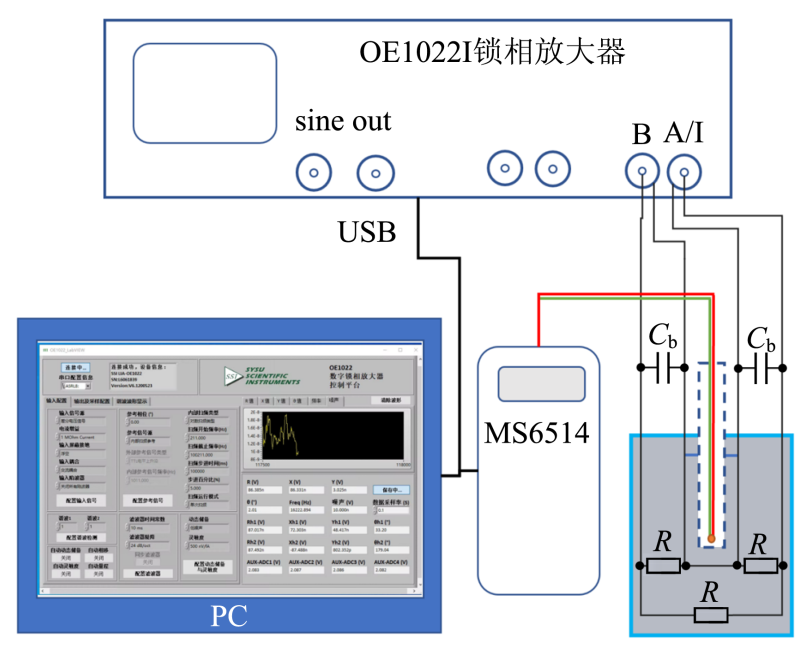
\includegraphics[width=0.5\linewidth]{images/APL1_1_A_connecting}
		\caption{电阻热噪声测量差分接线示意图（来自\cite{c}）}
		\label{fig:apl11aconnecting}
	\end{figure}
	
	仪器校正方面，此步骤中我们主要考虑\textbf{零点校正}。
	
	\item 选择仪器参数
	
	仪器的参数选择也主要参考实验讲义：
	
	\textbf{满量程灵敏度应选为 1$\mu$V；另一方面，热噪声幅值小，动态储备应选“Low Noise”。}
	
	由于测量装置不可能完全屏蔽环境干扰，选择太大的带宽容易引入近频的环境噪声，因此建议 Slope > 12dB/oct。
	
	为保证所采集的每个数据是独立的并且不失真，应该选择合适的采样的时间间隔。例如：当选时间常数 $\tau$ 为 30ms、Slope 为 18 dB/oct 时，ENBW 为 3/32 Hz，X 值的测量等待时间或时间间隔约为 $8.4\tau$（即 $\sim$250ms，见\cref{tab:ENBW}），X，Y 值同时采样 $10^3$ 个需要时间约为 4.5 分钟。
	
	由于缺乏具体实践经验，我们结合\cite{c}大胆给出一组可能的参数选取：98kΩ 电阻，在6666Hz下，$\tau=1s$，$\text{Slope}=24\text{dB/oct}$，时间间隔$10\tau$。
	
	\begin{ubox}{}
		事实上，上述参数设置存在不合理的地方，实际测量时我们选择了以下参数：
		\begin{itemize}
			\item 满量程灵敏度：1$\mu$V；
			
			\item 动态储备：“Low Noise”；
			
			\item 现场测量：$\tau = 10ms$，$\text{Slope} = 3/32$，$\Delta t_{sample}=0.1s$，频率点见\cref{fig:apl11aoriginaldata2}和\cref{fig:apl11aoriginaldata3}。
			
			\item 远程测量：$\tau = 100ms$，$\text{Slope} = 5/64$，$\Delta t_{sample}=1s$，频率点见\cref{fig:apl11adatapack}。
		\end{itemize}
	\end{ubox}
	
	\item 进行测量
	
	这个步骤中我们需要考虑\textbf{本底校正}。本底测量用 50Ω 短接，其余测量方式与所测热噪声的测量方式是相同的，注意如前文所述，本底校正一定是在选好参数后做的，换一组参数就要重做一次。
	
	接下来是正经的测量步骤，同样主要参考实验讲义。将上位 PC 机与锁相放大器相连，利用 OE1022 专用的 LabVIEW上位机采集程序对锁相放大器测量结果进行采样，采集当前锁相放大器测到的 X 值和 Y 值。采样间隔和保存路径在界面右上角 “sample” 选项卡中设置；锁相放大器参数在界面上方原理图内相关图标下的菜单中设置（这个示意图请看实验讲义）。
	
	总之，接线前和测量后请用万用表测量样品电阻， 以确认所在温度下其电阻值与标记的一致，并用于数据处理。在实验室先将线路接好； 分别打开所用锁相放大器的 LabVIEW 测量界面， 以及 MS6514 测温仪测量界面， 确认都可正常测量。 选择合适的仪器参数。 注意热电偶选“T 型” 。通过调节样品盒离液氮液面距离， 使样品自然稳定到某温度。
	
	\begin{ubox}{}
		具体来说，我们完成了以下测量：
		\begin{itemize}
			\item 现场本底噪声测量，共8组，与热噪声测量相对应。
			
			\item 现场热噪声测量，共8组，室温4组，低温4组。
			
			\item 结果如\cref{fig:apl11alocalmeasure1}和\cref{fig:apl11alocalmeasure2}所示。
		\end{itemize}
	\end{ubox}
	
	\item 远程测量
	
	与老师交流之后，我们进行了实验的远程测量。具体来说，由杨舒云22344020留在实验室在正式测量前保障接线等硬件设备能正常工作，由戴鹏辉22344016远程进行数据采集。
	
	远程测量热噪声，共8组，参数选择见前，均为进行本底噪声测量，结果如\cref{fig:apl11aremotemeasure1}和\cref{fig:apl11aremotemeasure2}所示。
\end{enumerate}	

% 实验结果
\subsubsection{Display}
\begin{enumerate}
	\item 现场测量
	
	现场测量时的实验软件界面截图和实际操作拍摄如\cref{fig:apl11alocalmeasure1}、\cref{fig:apl11alocalmeasure2}和\cref{fig:apl11alocalmeasure3}。
	
	\begin{figure}[h!]
		\centering
		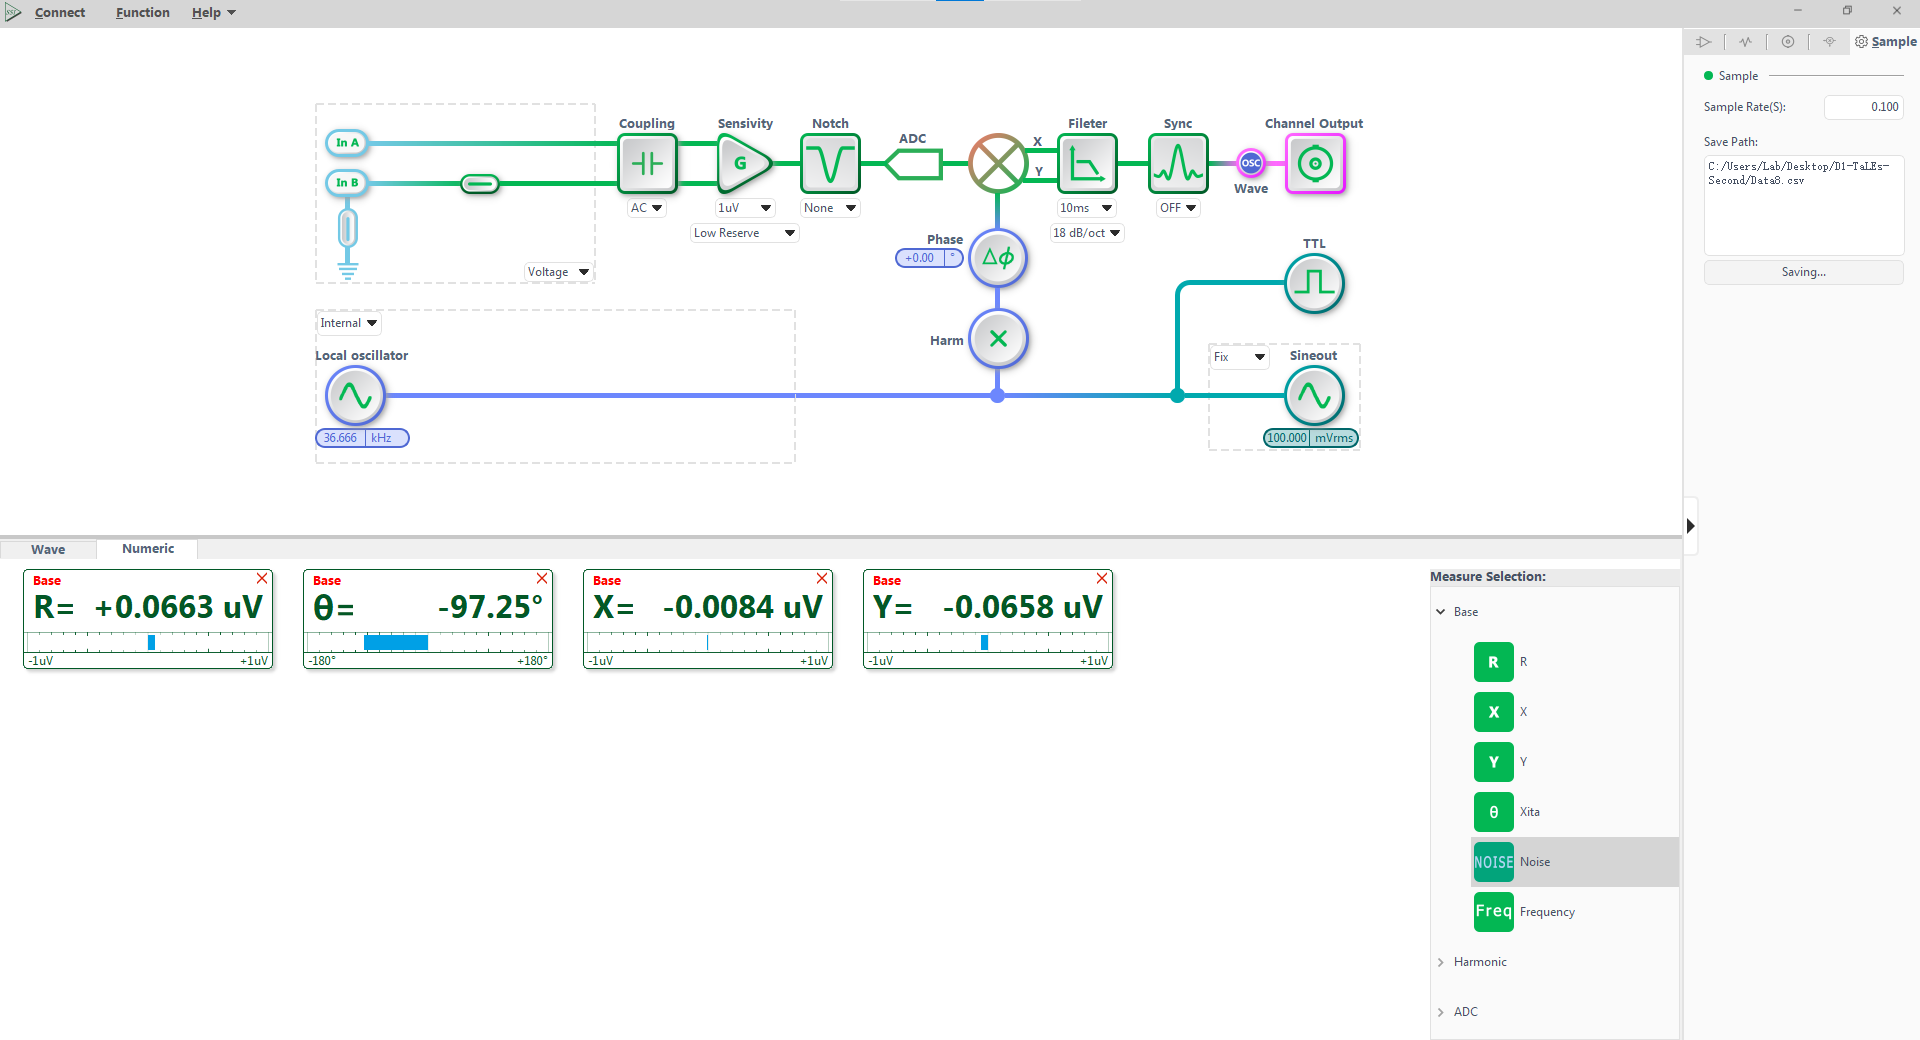
\includegraphics[width=0.5\linewidth]{images/APL1_1_A_local_measure1}
		\caption{现场测量1}
		\label{fig:apl11alocalmeasure1}
	\end{figure}
	
	\begin{figure}[h!]
		\centering
		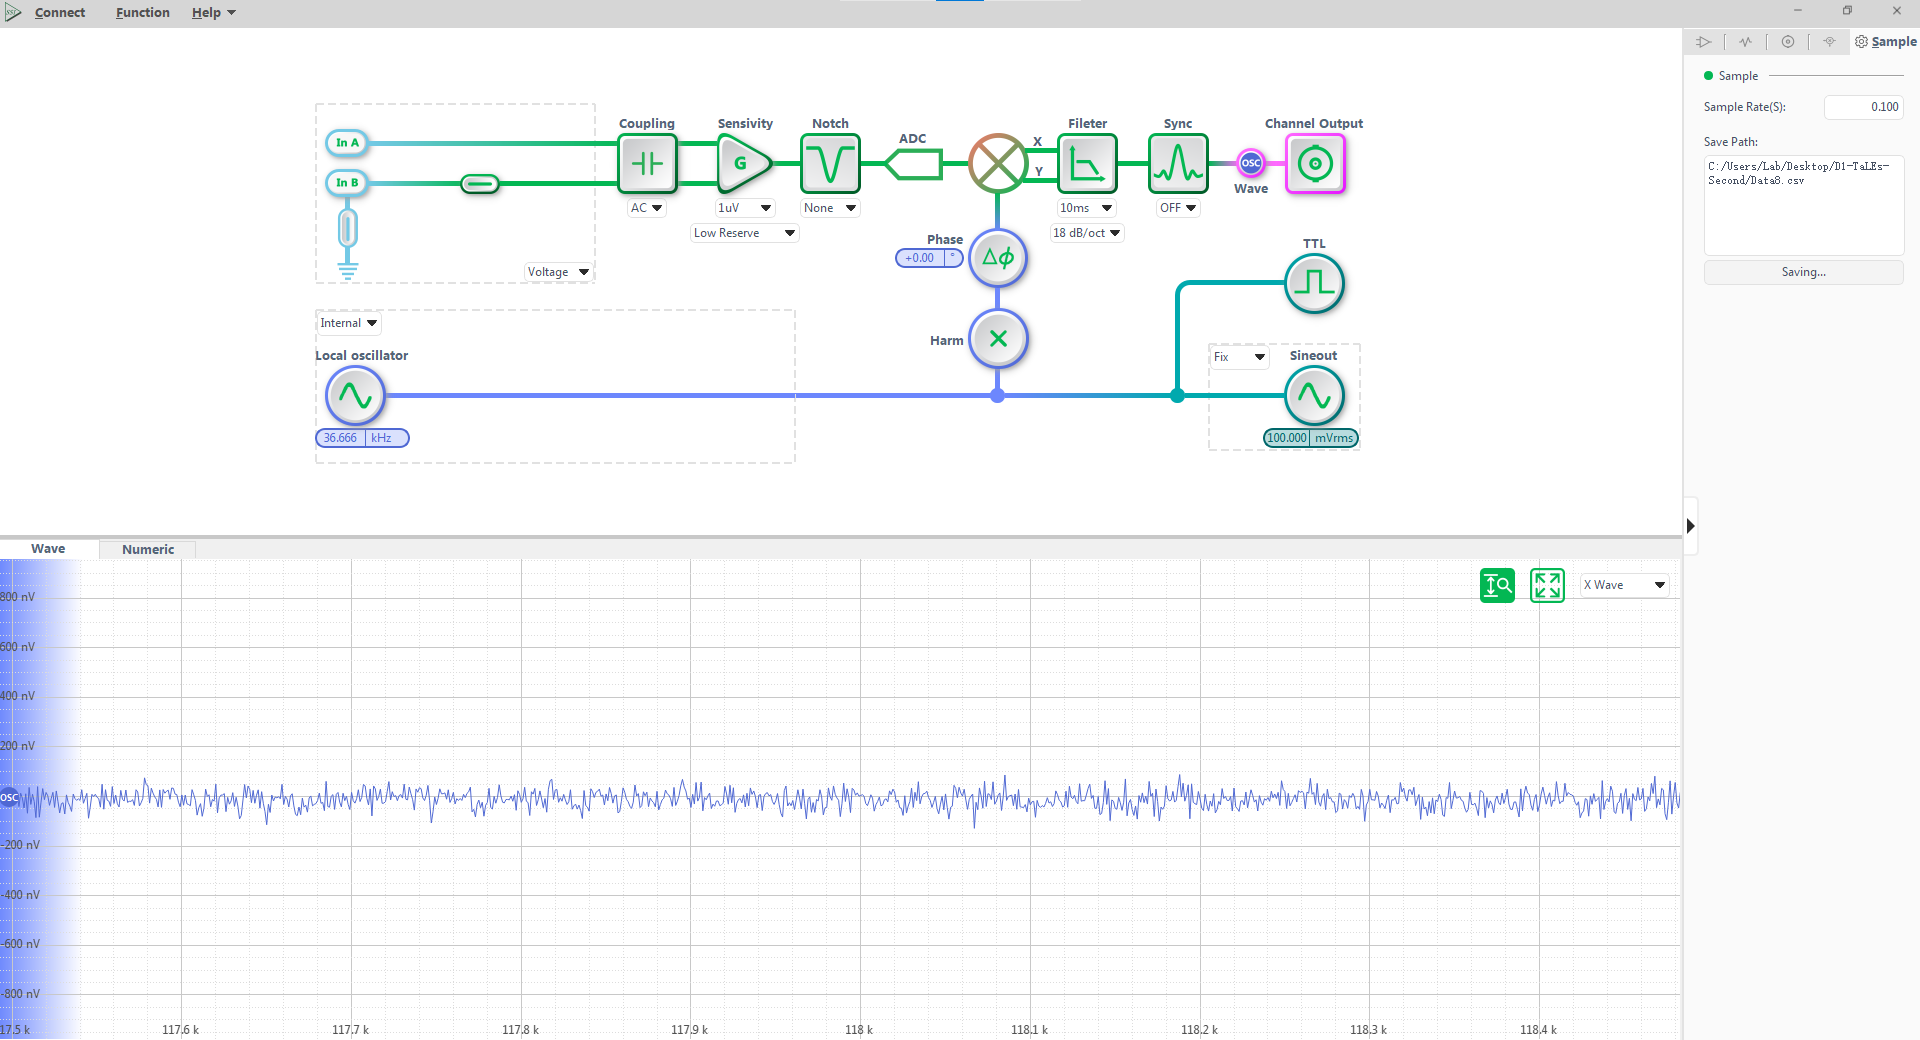
\includegraphics[width=0.5\linewidth]{images/APL1_1_A_local_measure2}
		\caption{现场测量2}
		\label{fig:apl11alocalmeasure2}
	\end{figure}

	\item 远程测量
	
	远程测量时的实验软件界面截图和实际操作拍摄如\cref{fig:apl11aremotemeasure1}、\cref{fig:apl11aremotemeasure2}和\cref{fig:apl11aremotemeasure3}。
	
	\begin{figure}[h!]
		\centering
		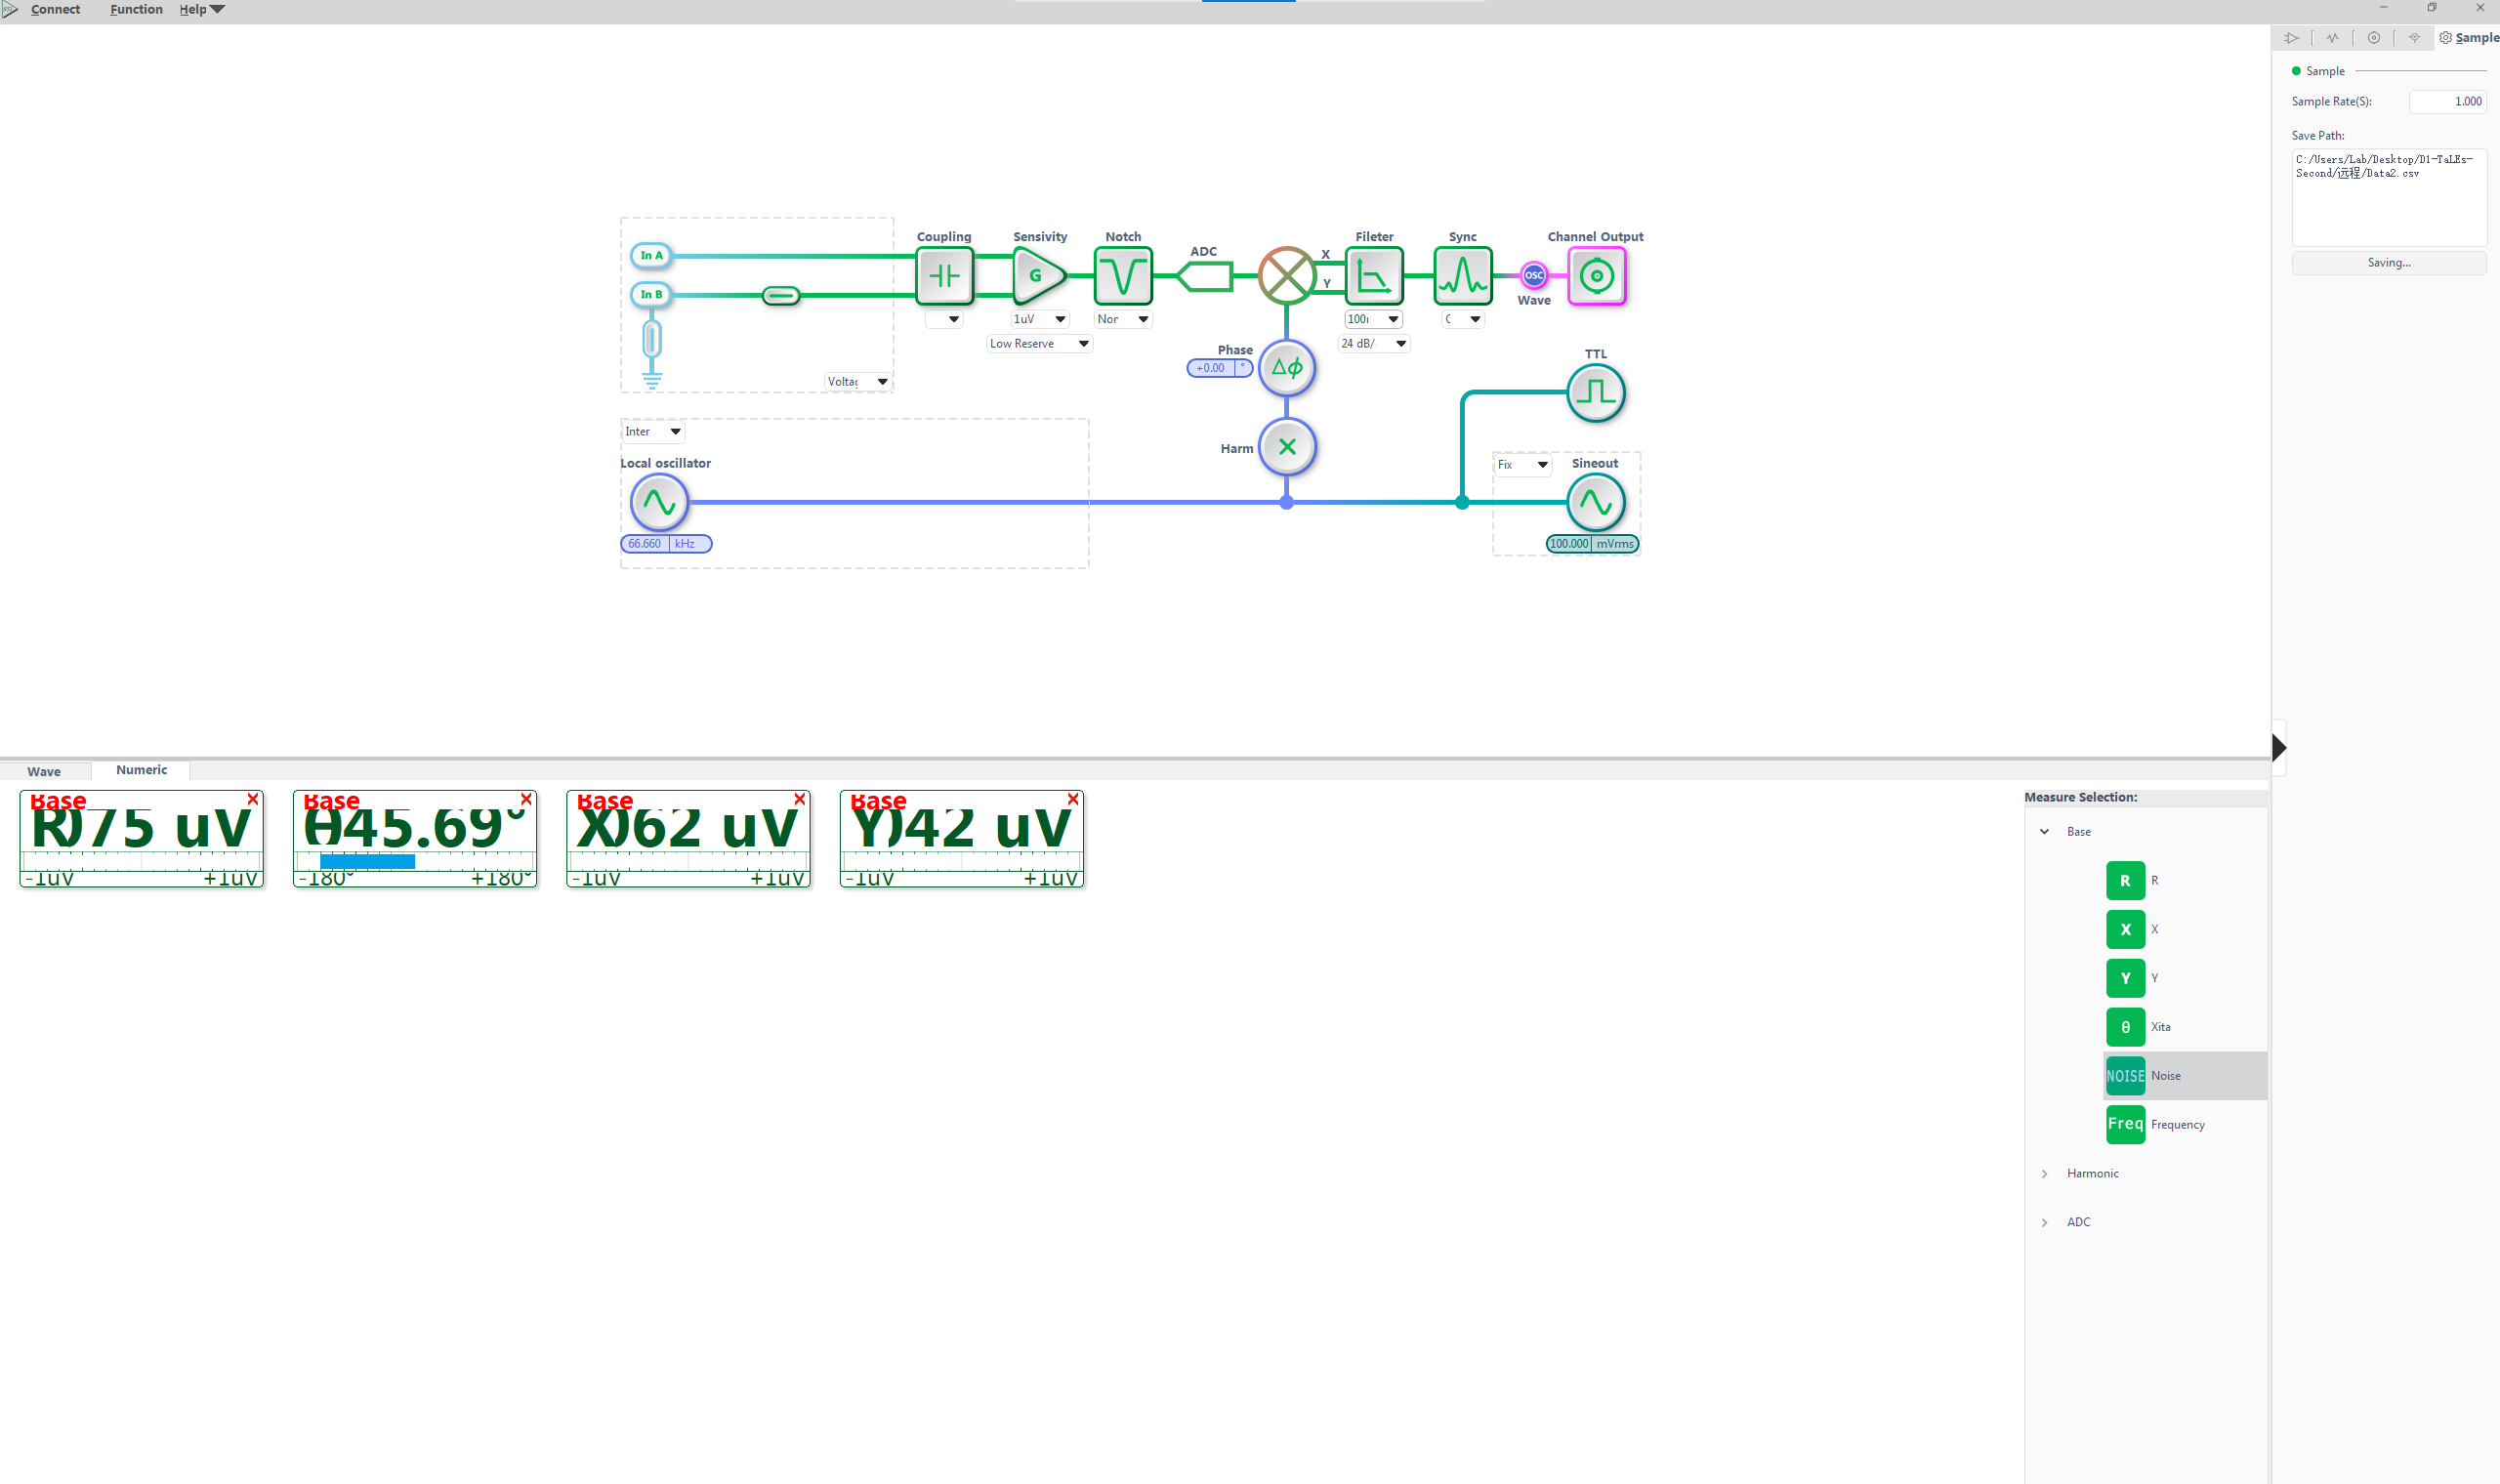
\includegraphics[width=0.5\linewidth]{images/APL1_1_A_remote_measure1}
		\caption{远程测量1}
		\label{fig:apl11aremotemeasure1}
	\end{figure}
	
	\begin{figure}[h!]
		\centering
		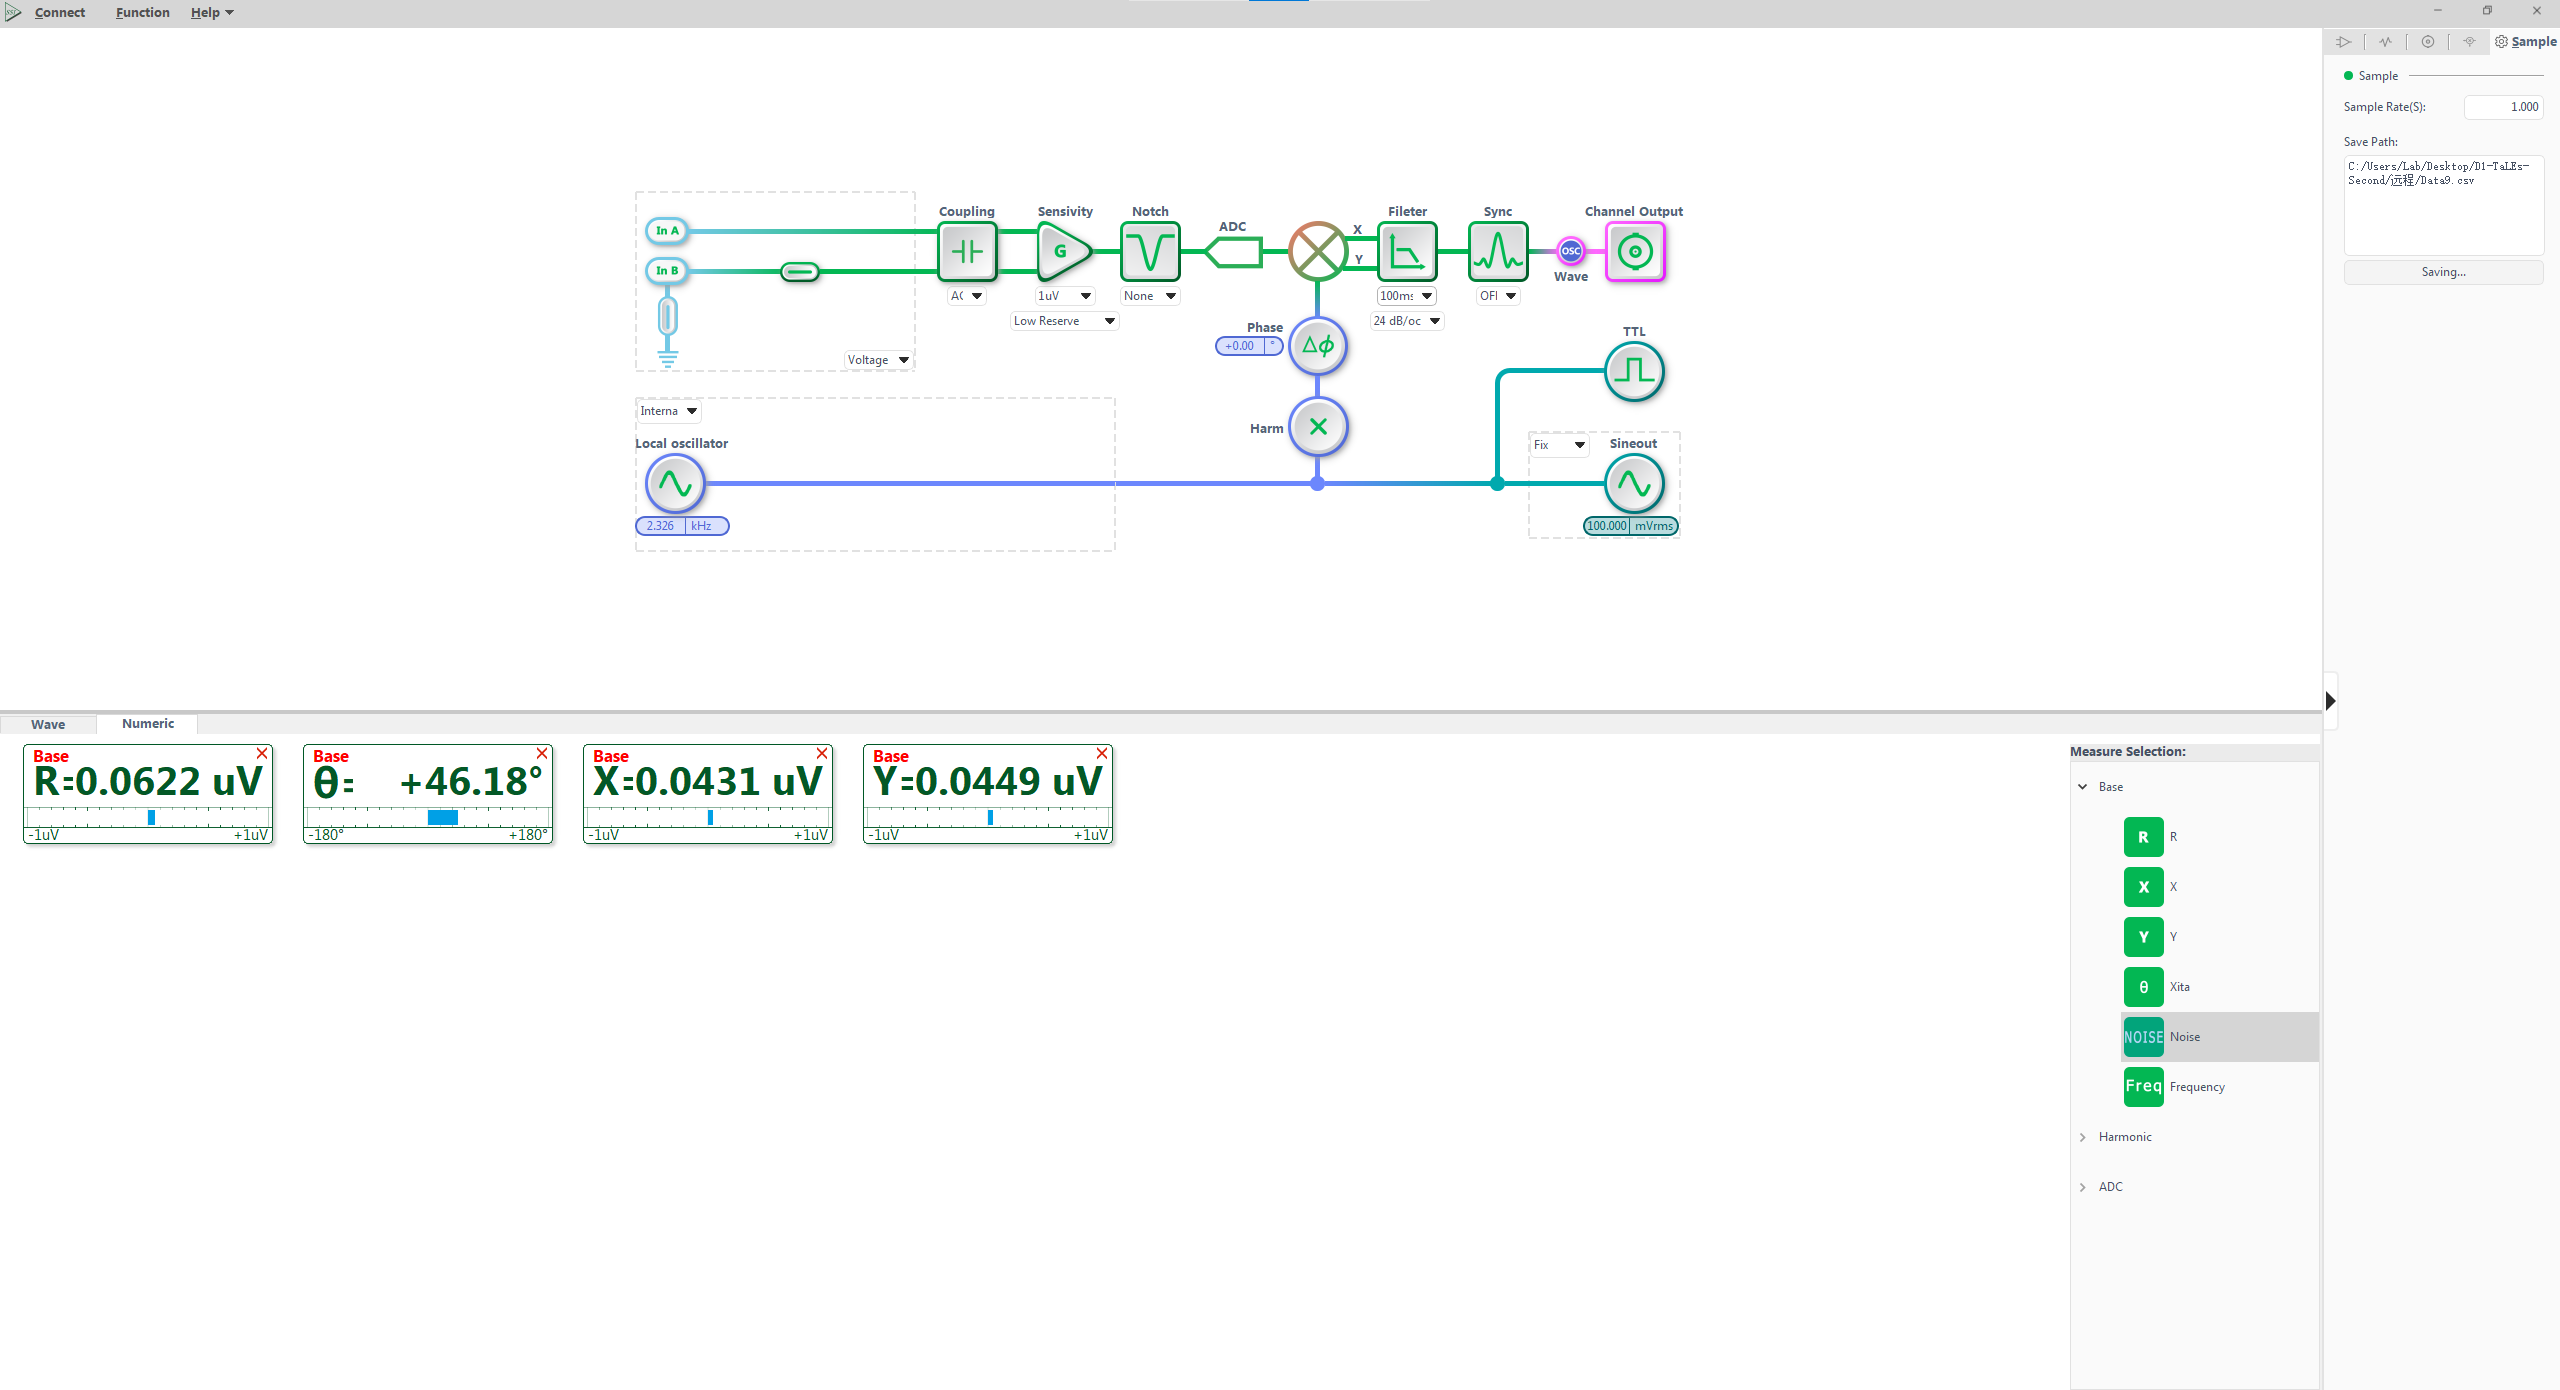
\includegraphics[width=0.5\linewidth]{images/APL1_1_A_remote_measure2}
		\caption{远程测量2}
		\label{fig:apl11aremotemeasure2}
	\end{figure}
	
	\item 实验数据
	\begin{itemize}
		\item 实验数据清单：
		\begin{enumerate}
			\item 本地测量热噪声原始数据：文件夹“\texttt{data-set/local}”；
			\item 本地测量本底噪声原始数据：文件夹“\texttt{data-set/base}”；
			\item 远程测量热噪声原始数据：文件夹“\texttt{data-set/remote}”；
			\item 原始数据手写记录：文件夹“\texttt{origin}”；
			\item 数据汇总表：文件“\texttt{APL1\_1\_A\_data\_tabel.slsx}”；
			\item 原始数据说明文件（参数信息记录）：文件夹“\texttt{directions}”。
		\end{enumerate}
		
		\item 上述实验数据已经打包为zip并上传seelight相应位置。
		
		\begin{figure}[h!]
			\centering
			\includegraphics[width=0.5\linewidth]{images/APL1_1_A_datapack}
			\caption{实验数据包}
			\label{fig:apl11adatapack}
		\end{figure}
		
	\end{itemize}
	
\end{enumerate}

%---------------------------------------------------------------------
% 原始数据
\subsection{Original Data}
The original data in the experimental notebook is shown in \cref{fig:apl11aoriginaldata1},  \cref{fig:apl11aoriginaldata2} and \cref{fig:apl11aoriginaldata3} (signed).

\begin{figure}[h!]
	\centering
	\includegraphics[width=0.5\linewidth]{images/APL1_1_A_original_data1}
	\caption{原始数据1}
	\label{fig:apl11aoriginaldata1}
\end{figure}

\begin{figure}[h!]
	\centering
	\includegraphics[width=0.5\linewidth]{images/APL1_1_A_original_data2}
	\caption{原始数据2}
	\label{fig:apl11aoriginaldata2}
\end{figure}

\begin{figure}[h!]
	\centering
	\includegraphics[width=0.5\linewidth]{images/APL1_1_A_original_data3}
	\caption{原始数据3}
	\label{fig:apl11aoriginaldata3}
\end{figure}

Other raw data are shown in \cref{fig:apl11alocalmeasure1}, \cref{fig:apl11alocalmeasure2}, \cref{fig:apl11aremotemeasure1}, \cref{fig:apl11aremotemeasure2} and \cref{fig:apl11adatapack}.

%---------------------------------------------------------------------
%% 问题记录
%\subsection{Difficulties}
%\begin{enumerate}
%	\item 
%\end{enumerate}